\documentclass{beamer}
\usetheme{Boadilla}
%Information to be included in the title page:
\title[Eco B] %optional
{When scale and replication work: Learning from summer youth
employment experiments - Discussion}

\subtitle{Paper by Sara B. Heller}

\author % (optional, for multiple authors)
{Daniel Pollak}

\institute[TAU] % (optional)
{
  Tel-Aviv University
}

\date{Jun 2023}

\begin{document}

\frame{\titlepage}

\begin{frame}
\frametitle{Overview}
\begin{itemize}
  \item \textbf{Main questions:}
  \begin{itemize}
    \item What is the effect of summer youth employment programs on socialy bad behavior?
    \item What are the heterogeneous effects of these programs?
  \end{itemize}
  \item \textbf{Data:}
  \begin{itemize}
    \item RCT of OSC+ in Chicago, and WorkReady in Philadelphia
    \item WorkReady served a less targeted, less criminally active population than OSC+
    \item Administrative data on youth
    contact with various government agencies, arrests records, and so on..
  \end{itemize}
\end{itemize}

\end{frame}

\begin{frame}
\frametitle{Empirical Strategy Reiteration}
$$Y_{ist}=\beta_0+\beta_1T_{is}+B_2X_{ist-1}+\gamma_s+\epsilon_{ist}$$
\begin{itemize}
  \item $i$ - individual, $s$ - strata (program) location, $t$ - period
  \item $Y_{ist}$ captures the outcome of interest for the individual, $T_{is}$ is an indicator for individual i being randomly assigned to be offered a program, $X_{ist-1}$ is a set of
  individual i’s pre-randomization characteristics
  \item Identifies ITT - the effect of receiving the option to participate in a program
  \item Using $T_{is}$ as instrument for paticipation identifies LATE - the effect for the compliers
\end{itemize}
\end{frame}

\begin{frame}
  \frametitle{Assumptions}
  All assumptions hold trivially due to the random assignment
\end{frame}

\begin{frame}
\frametitle{Results}

\begin{table}[!htbp] \centering 
  \label{} 
\begin{tabular}{@{\extracolsep{5pt}}lcccc} 
\hline \\
[-1.8ex] & ITT & Control-mean & LATE \\ 
\hline \\[-1.8ex] 
 & \multicolumn{3}{c}{\textit{WorkReady}} \\ 
\cline{2-4} \\
Total Number of Arrests & -.010$^{**}$ & 0.028 & -0.030$^{**}$ \\ 
  & (0.003) & & (0.0009) \\
Number of Other Arrests & -.004$^{**}$ & 0.004 & -0.011$^{**}$ \\ 
  & (0.001) & & (0.004) \\
\cline{2-4} \\
[-1.8ex] & \multicolumn{3}{c}{\textit{OCS+}} \\ 
\cline{2-4} \\
Total Number of Arrests & -0.023 & 0.176 & -0.087 \\ 
  & (0.015) & & (0.057) \\
Number of Other Arrests & -0.017$^{*}$ & 0.084 & -0.063$^{*}$ \\ 
& (0.009) & & (0.035) \\
\hline
\end{tabular}
\end{table}
The higher the control-means, the stronger the effect?
\end{frame}

\begin{frame}
\frametitle{Discussion}
\begin{itemize}
\item The paper estimates effect heterogeneity by counterfactual outcome level
\item Varitation in $Y_{i0}$ represents the risk of the individual
\begin{itemize}
  \item Higher is riskier
\end{itemize}
\item $Y_0$ is not observed for the treatment group
\item Comparing LATE from multiple experiments as function of control means
\end{itemize}
\begin{figure}
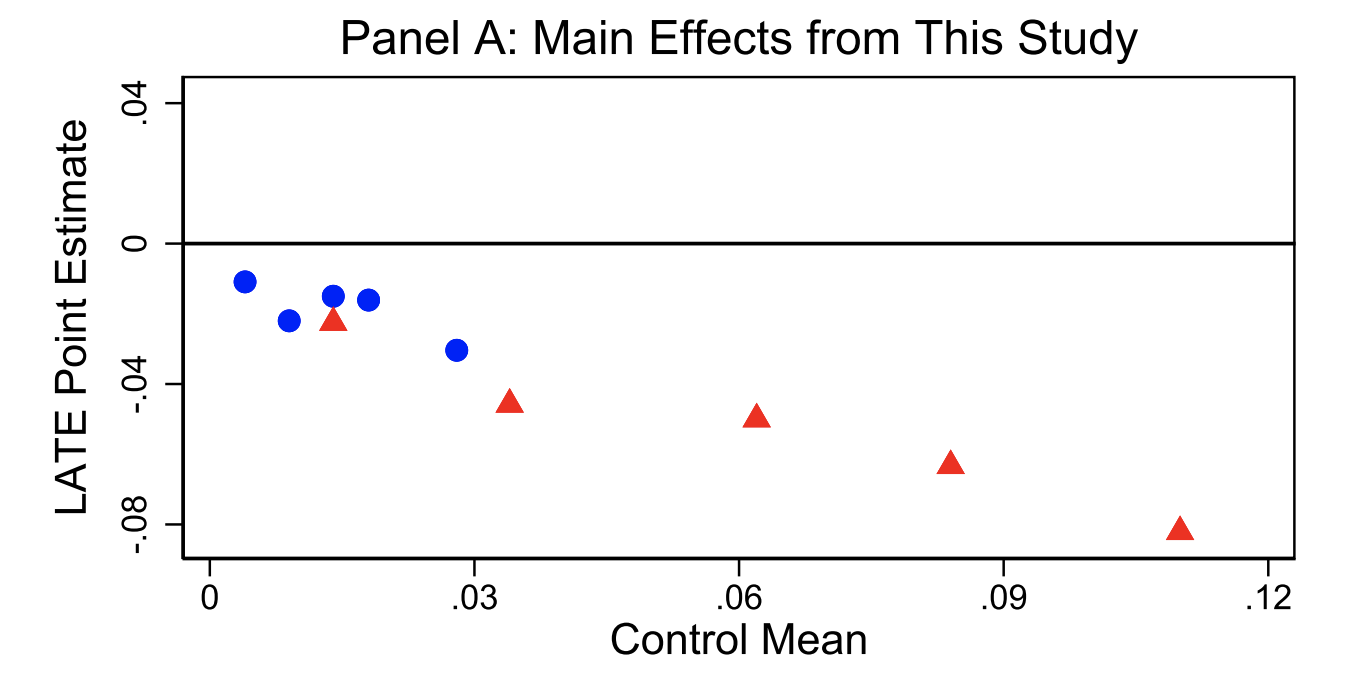
\includegraphics[width=6cm]{fig/fig2.png}
\end{figure}
\end{frame}

\begin{frame}
\frametitle{Discussion}
\begin{itemize}
\item  We might extrapolate the absolute magnitude of SYEPs’ effects in new settings as a proportional function of the anticipated control mean
\item But there could be other explanations -
\begin{itemize}
  \item Focusing specific level of risk in the participants (OSC+ targets more violent people)
  \item Low risk individuals may have benefitted from other programs or support
\end{itemize}
\item Anything correlated with higher $Y_0$s, including program design and implementation details that differ for higher-risk groups, could be driving the relationship
\end{itemize}
\end{frame}

\end{document}